% mnras_template.tex
%
% LaTeX template for creating an MNRAS paper
%
% v3.0 released 14 May 2015
% (version numbers match those of mnras.cls)
%
% Copyright (C) Royal Astronomical Society 2015
% Authors:
% Keith T. Smith (Royal Astronomical Society)

% Change log
%
% v3.0 May 2015
%    Renamed to match the new package name
%    Version number matches mnras.cls
%    A few minor tweaks to wording
% v1.0 September 2013
%    Beta testing only - never publicly released
%    First version: a simple (ish) template for creating an MNRAS paper

%%%%%%%%%%%%%%%%%%%%%%%%%%%%%%%%%%%%%%%%%%%%%%%%%%
% Basic setup. Most papers should leave these options alone.
\documentclass[a4paper,fleqn,usenatbib]{mnras}

% MNRAS is set in Times font. If you don't have this installed (most LaTeX
% installations will be fine) or prefer the old Computer Modern fonts, comment
% out the following line
\usepackage{newtxtext,newtxmath}
% Depending on your LaTeX fonts installation, you might get better results with one of these:
%\usepackage{mathptmx}
%\usepackage{txfonts}

% Use vector fonts, so it zooms properly in on-screen viewing software
% Don't change these lines unless you know what you are doing
\usepackage[T1]{fontenc}
\usepackage{ae,aecompl}


%%%%% AUTHORS - PLACE YOUR OWN PACKAGES HERE %%%%%

% Only include extra packages if you really need them. Common packages are:
\usepackage{graphicx}	% Including figure files
\usepackage{amsmath}	% Advanced maths commands
\usepackage{amssymb}	% Extra maths symbols

%%%%%%%%%%%%%%%%%%%%%%%%%%%%%%%%%%%%%%%%%%%%%%%%%%

%%%%% AUTHORS - PLACE YOUR OWN COMMANDS HERE %%%%%

% Please keep new commands to a minimum, and use \newcommand not \def to avoid
% overwriting existing commands. Example:
%\newcommand{\pcm}{\,cm$^{-2}$}	% per cm-squared

%%%%%%%%%%%%%%%%%%%%%%%%%%%%%%%%%%%%%%%%%%%%%%%%%%

%%%%%%%%%%%%%%%%%%% TITLE PAGE %%%%%%%%%%%%%%%%%%%

% Title of the paper, and the short title which is used in the headers.
% Keep the title short and informative.
\title[Short title, max. 45 characters]{MNRAS \LaTeXe\ template -- title goes here}

% The list of authors, and the short list which is used in the headers.
% If you need two or more lines of authors, add an extra line using \newauthor
\author[K. T. Smith et al.]{
Keith T. Smith,$^{1}$\thanks{E-mail: mn@ras.org.uk (KTS)}
A. N. Other,$^{2}$
Third Author$^{2,3}$
and Fourth Author$^{3}$
\\
% List of institutions
$^{1}$Royal Astronomical Society, Burlington House, Piccadilly, London W1J 0BQ, UK\\
$^{2}$Department, Institution, Street Address, City Postal Code, Country\\
$^{3}$Another Department, Different Institution, Street Address, City Postal Code, Country
}

% These dates will be filled out by the publisher
\date{Accepted XXX. Received YYY; in original form ZZZ}

% Enter the current year, for the copyright statements etc.
\pubyear{2015}

% Don't change these lines
\begin{document}
\label{firstpage}
\pagerange{\pageref{firstpage}--\pageref{lastpage}}
\maketitle

% Abstract of the paper
\begin{abstract}
This is a simple template for authors to write new MNRAS papers.
The abstract should briefly describe the aims, methods, and main results of the paper.
It should be a single paragraph not more than 250 words (200 words for Letters).
No references should appear in the abstract.
\end{abstract}

% Select between one and six entries from the list of approved keywords.
% Don't make up new ones.
\begin{keywords}
keyword1 -- keyword2 -- keyword3
\end{keywords}

%%%%%%%%%%%%%%%%%%%%%%%%%%%%%%%%%%%%%%%%%%%%%%%%%%

%%%%%%%%%%%%%%%%% BODY OF PAPER %%%%%%%%%%%%%%%%%%

\section{Introduction}

This is a simple template for authors to write new MNRAS papers.
See \texttt{mnras\_sample.tex} for a more complex example, and \texttt{mnras\_guide.tex}
for a full user guide.

All papers should start with an Introduction section, which sets the work
in context, cites relevant earlier studies in the field by \citet{Others2013},
and describes the problem the authors aim to solve \citep[e.g.][]{Author2012}.

\section{Illustris Simulation}
Illustris-1, also known simply as Illustris, is a highly resolved cosmological simulation which reproduces large-scale statistical features of the Universe, such as the galaxy population of massive clusters, as well as small-scale properties such as the morphology of galaxies and detailed values for their stellar and gas content. This was achieved by following the evolution of $1820^3$ DM particles with mass resolution $m_{\text{DM}} = 6.26\cdot 10^6\text{M}_{\odot}$, together with $1820^3$ baryonic particles with mass resolution $\overline{\text{m}_\text{b}}=1.26\cdot 10^6\text{M}_{\odot}$ from a glass-like configuration, in a periodic box of $106.5\text{Mpc}$, all of which is consistent with a standard $\Lambda \text{CDM}$ cosmology with $\Omega_\Lambda=0.7274$, $\Omega_\text{m}=0.2726$, $\Omega_\text{b}=0.0456$, $\sigma_\text{s}=0.0.809$, $\text{n}_\text{s}=0.963$ \& $\text{H}_0=70.4\text{kms}
^{-1}\text{Mpc}^{-1}$. Illustris has a constant spatial resolution of $1.4\text{kpc}$ for DM particles in comoving units, and for baryonic particles it has the same spatial resolution of DM for $\text{z}\geq 1$, which is later modified to $0.7\text{kpc}$ in physical units for the rest of the simulation. The evolution in time was performed with the hydrodynamic algorithm AREPO \cite{arepo}, which combines a moving Voronoi tessellation with the finite volume approach. Included in the evolution algorithm, there are galaxy formation models which account for the evolution of stars and SMBHs. The level of detail in Illustris is advantageous and hard to find among other simulations, and is the reason why we chose it to perform our calculations.\\

This simulation consists of 136 snapshots where 61 of them were taken at $z < 3$ spaced with a cosmological scale factor $\Delta a \approx 0.02$, while the remaining 75 were taken at $z > 3$ with spacing $\Delta a \approx 0.01$. Each snapshot was post-processed with modified versions of FOF and SUBFIND algorithms \cite{fof,subfind} to generate halo and subhalo catalogues with their respective characterization properties.  

\section{The method}
The principal purpose of this work is to verify if the results obtained observationally by Jones et al. \cite{jones1} are supported by a similar analysis in the cosmological simulation Illustris. For this purpose, we want to adaptate the observational method as closely as posible for it to work on computational data.\\

The principal method used in Jones et al. \cite{jones1} for the analysis of the dependence of the Schechter parameters on the cosmological environment is as follows. To obtain a quantification of environment, they calculated for, each galaxy in the studied survey, the projected distance in the sky to the third nearest neighbor, filtrating candidate galaxies by its radial velocity relative to the galaxy studied. According to Hubble's law, this effectively restricts the candidate galaxies to a smaller radial range, reducing apparent closer galaxies arising from the projection method. The radial relative velocity cut was chosen to be $450km/s$. Furthermore, a photometrics preselection was performed, selecting galaxies whose r-filter magnitude was above $-19$ (VERIFY).\\

Once quantified the environment with the distance to the 3rd nearest neighbor definition for each galaxy in their post-selected survey they divided the group in four quartiles according this quantity. For each quartile, the respective HIMF was calculated, and with this, a Schechter fit was obtained. The analysis was specifically performed over the Schechter parameters of the Knee-mass and the faint-end slope.\\

In dark matter cosmological simulations, acces to the information is istantaneous and at no cost. However, as we want to replicate as closely as possible the method effectuated by Jones et. al \cite{jones1}. We also calculate the projected distance in the simulation, according to a specified point of view, taking the same radial velocity cut having into account distance and peculiar velocities. Even when we could easily calculate the distance to the third nearest neighbor we take into account these observational simplifications, to make our study as comparable as possible to that of Jones et al. \cite{jones1}

\section{Results}
\subsection{Preliminaries}

\subsection{Mass functions comparison}

Figures and tables should be placed at logical positions in the text. Don't
worry about the exact layout, which will be handled by the publishers.

Figures are referred to as e.g. Fig.~\ref{fig:example_figure}, and tables as
e.g. Table~\ref{tab:example_table}.

% Quartiles gas
\begin{figure}
	% To include a figure from a file named example.*
	% Allowable file formats are eps or ps if compiling using latex
	% or pdf, png, jpg if compiling using pdflatex
	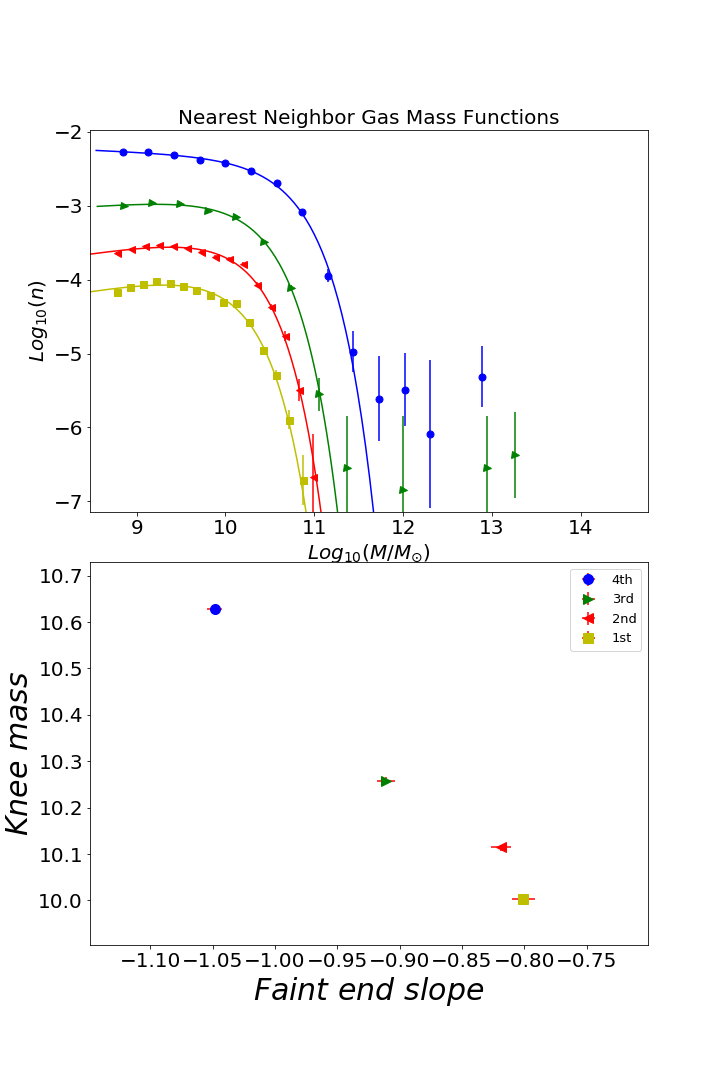
\includegraphics[width=\columnwidth]{./pics/quartilesGas.png}
    \caption{\textbf{Upper side}: Schechter fits of each gas mass function for each environmental quartile using the 3rd nearest neighbor definition.\textbf{Down side}: Knee-mass $m_\ast$ and the faint end slope $\alpha$ values obtained from the Schechter fits for each curve shown above.}
    \label{fig:quartilesGas}
\end{figure}

% Tweb gas
\begin{figure}
	% To include a figure from a file named example.*
	% Allowable file formats are eps or ps if compiling using latex
	% or pdf, png, jpg if compiling using pdflatex
	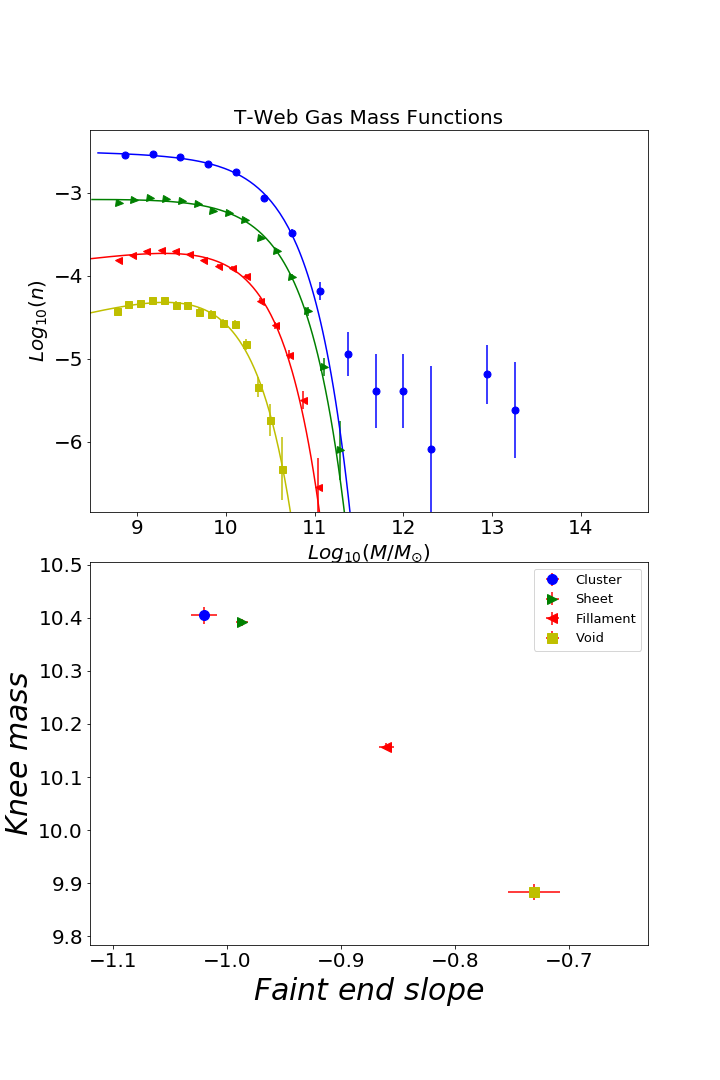
\includegraphics[width=\columnwidth]{./pics/T-Web_Gas.png}
    \caption{\textbf{Upper side}: Schechter fits of each gas mass function for each morphological environment characterized by the T-Web algorithm proposed by Forero et al.\textbf{Down side}: Knee-mass $m_\ast$ and the faint end slope $\alpha$ values obtained from the Schechter fits for each curve shown above.}
    \label{fig:TwebGas}
\end{figure}

% Quartiles DM
\begin{figure}
	% To include a figure from a file named example.*
	% Allowable file formats are eps or ps if compiling using latex
	% or pdf, png, jpg if compiling using pdflatex
	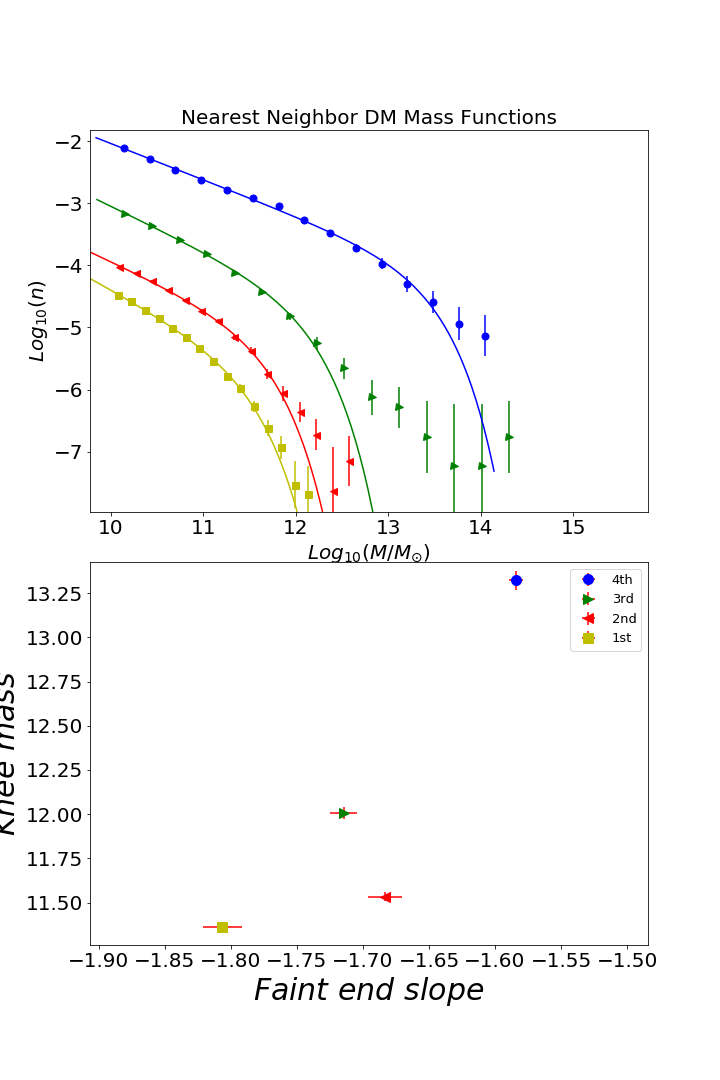
\includegraphics[width=\columnwidth]{./pics/quartilesDM.png}
    \caption{\textbf{Upper side}: Schechter fits of each DM mass function for each environmental quartile using the 3rd nearest neighbor definition.\textbf{Down side}: Knee-mass $m_\ast$ and the faint end slope $\alpha$ values obtained from the Schechter fits for each curve shown above.}
    \label{fig:quartilesDM}
\end{figure}

% Tweb DM
\begin{figure}
	% To include a figure from a file named example.*
	% Allowable file formats are eps or ps if compiling using latex
	% or pdf, png, jpg if compiling using pdflatex
	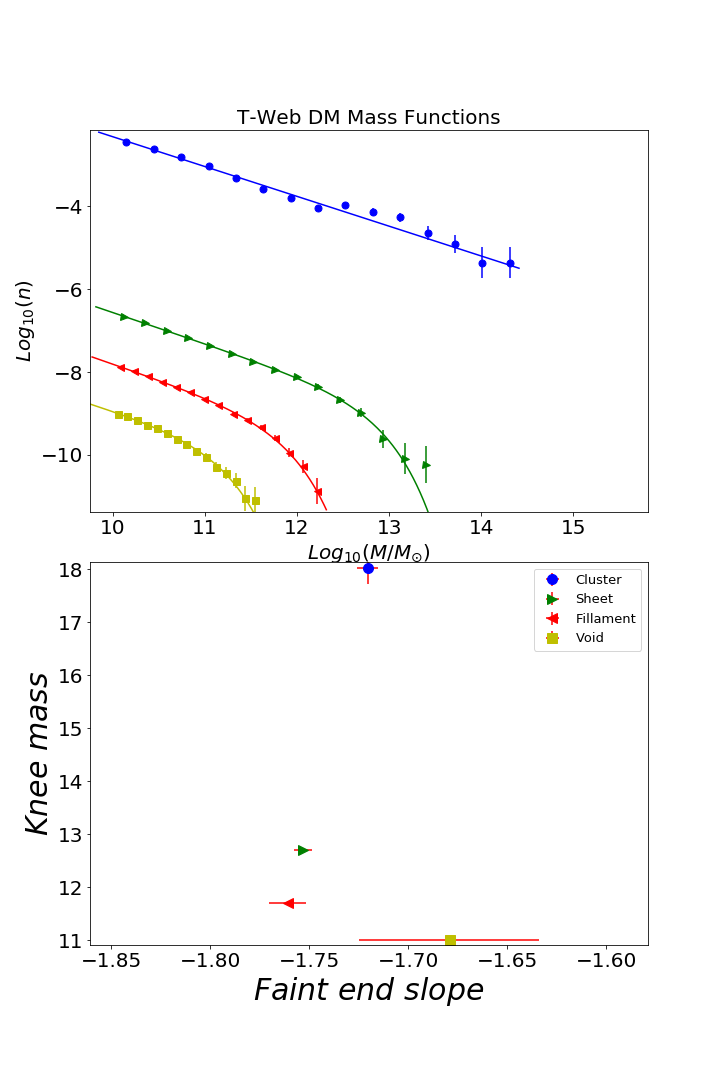
\includegraphics[width=\columnwidth]{./pics/T-Web_DM.png}
    \caption{\textbf{Upper side}: Schechter fits of each DM mass function for each morphological environment characterized by the T-Web algorithm proposed by Forero et al.\textbf{Down side}: Knee-mass $m_\ast$ and the faint end slope $\alpha$ values obtained from the Schechter fits for each curve shown above.}
    \label{fig:TwebDM}
\end{figure}

% Quartiles Stellar
\begin{figure}
	% To include a figure from a file named example.*
	% Allowable file formats are eps or ps if compiling using latex
	% or pdf, png, jpg if compiling using pdflatex
	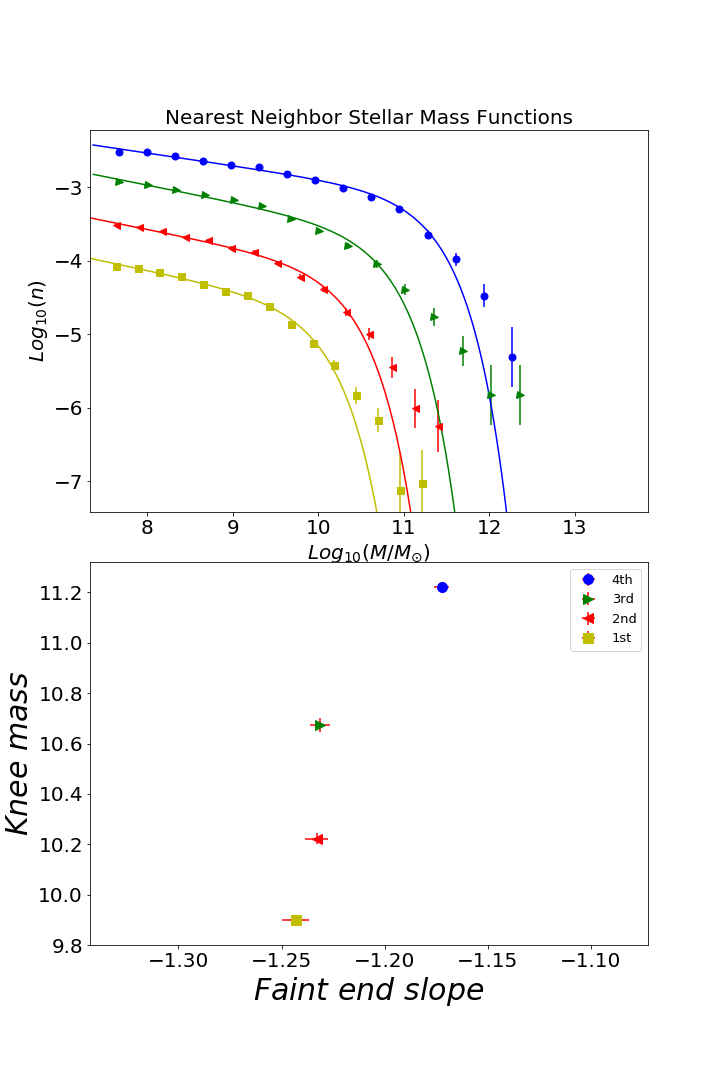
\includegraphics[width=\columnwidth]{./pics/quartilesSellar.png}
    \caption{\textbf{Upper side}: Schechter fits of each stellar mass function for each environmental quartile using the 3rd nearest neighbor definition.\textbf{Down side}: Knee-mass $m_\ast$ and the faint end slope $\alpha$ values obtained from the Schechter fits for each curve shown above.}
    \label{fig:quartilesStellar}
\end{figure}

% Tweb Stellar
\begin{figure}
	% To include a figure from a file named example.*
	% Allowable file formats are eps or ps if compiling using latex
	% or pdf, png, jpg if compiling using pdflatex
	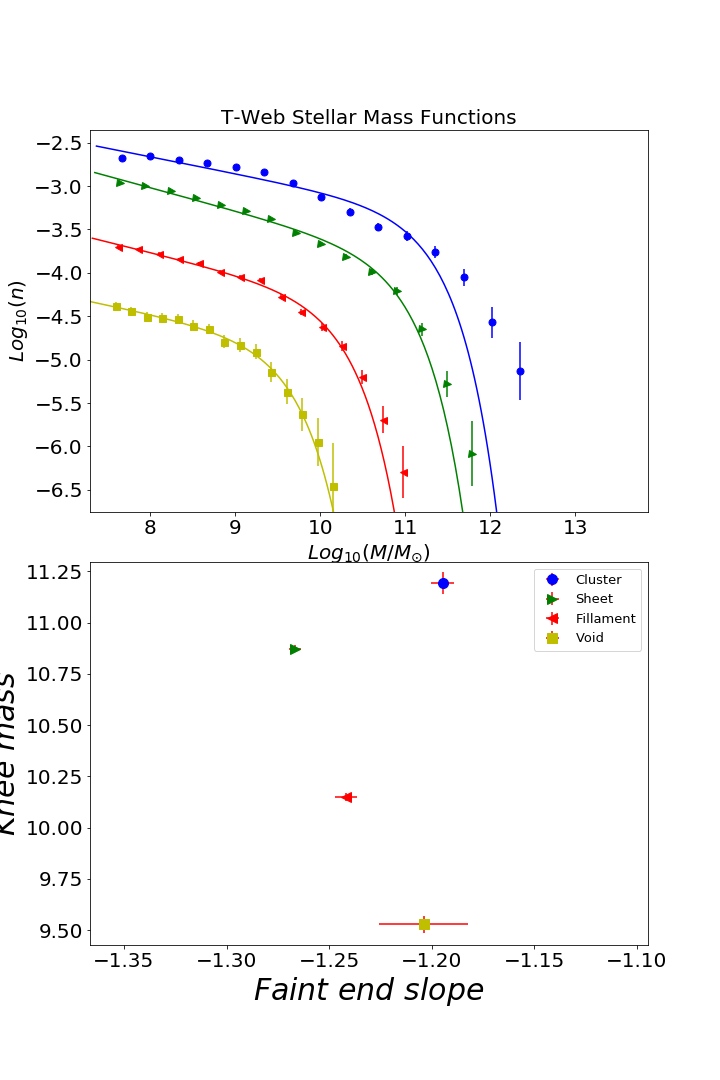
\includegraphics[width=\columnwidth]{./pics/T-Web_Stellar.png}
    \caption{\textbf{Upper side}: Schechter fits of each stellar mass function for each morphological environment characterized by the T-Web algorithm proposed by Forero et al.\textbf{Down side}: Knee-mass $m_\ast$ and the faint end slope $\alpha$ values obtained from the Schechter fits for each curve shown above.}
    \label{fig:TwebStellar}
\end{figure}

% Quartiles BH
\begin{figure}
	% To include a figure from a file named example.*
	% Allowable file formats are eps or ps if compiling using latex
	% or pdf, png, jpg if compiling using pdflatex
	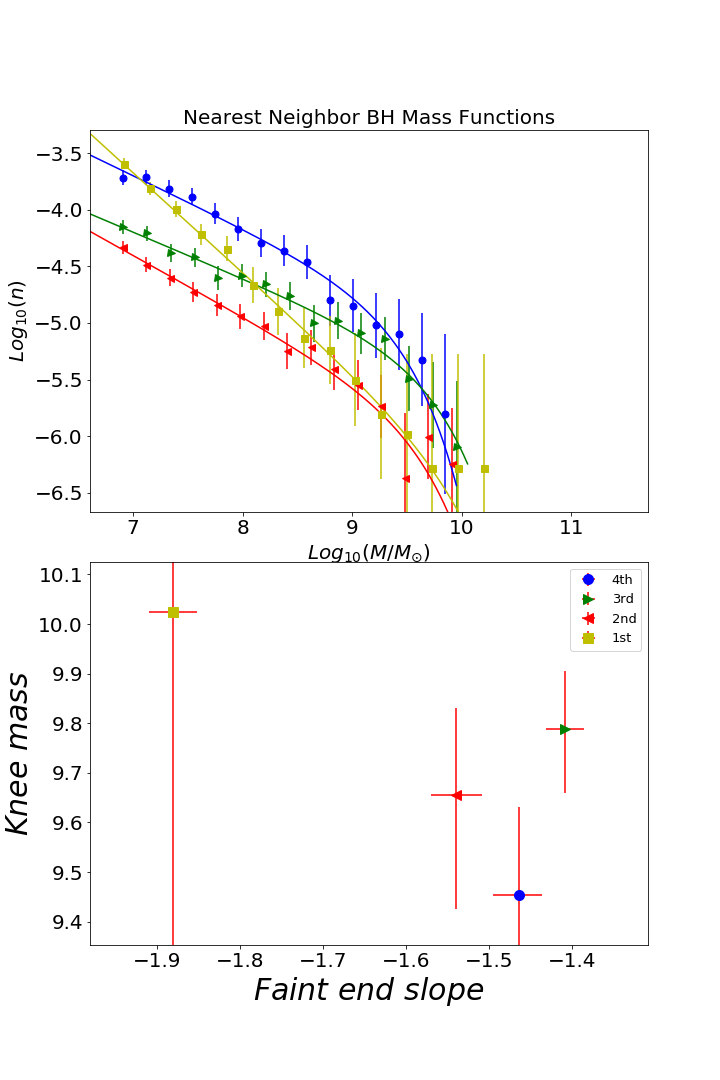
\includegraphics[width=\columnwidth]{./pics/quartilesBH.png}
    \caption{\textbf{Upper side}: Schechter fits of each BH mass function for each environmental quartile using the 3rd nearest neighbor definition.\textbf{Down side}: Knee-mass $m_\ast$ and the faint end slope $\alpha$ values obtained from the Schechter fits for each curve shown above.}
    \label{fig:quartilesBH}
\end{figure}

% Tweb BH
\begin{figure}
	% To include a figure from a file named example.*
	% Allowable file formats are eps or ps if compiling using latex
	% or pdf, png, jpg if compiling using pdflatex
	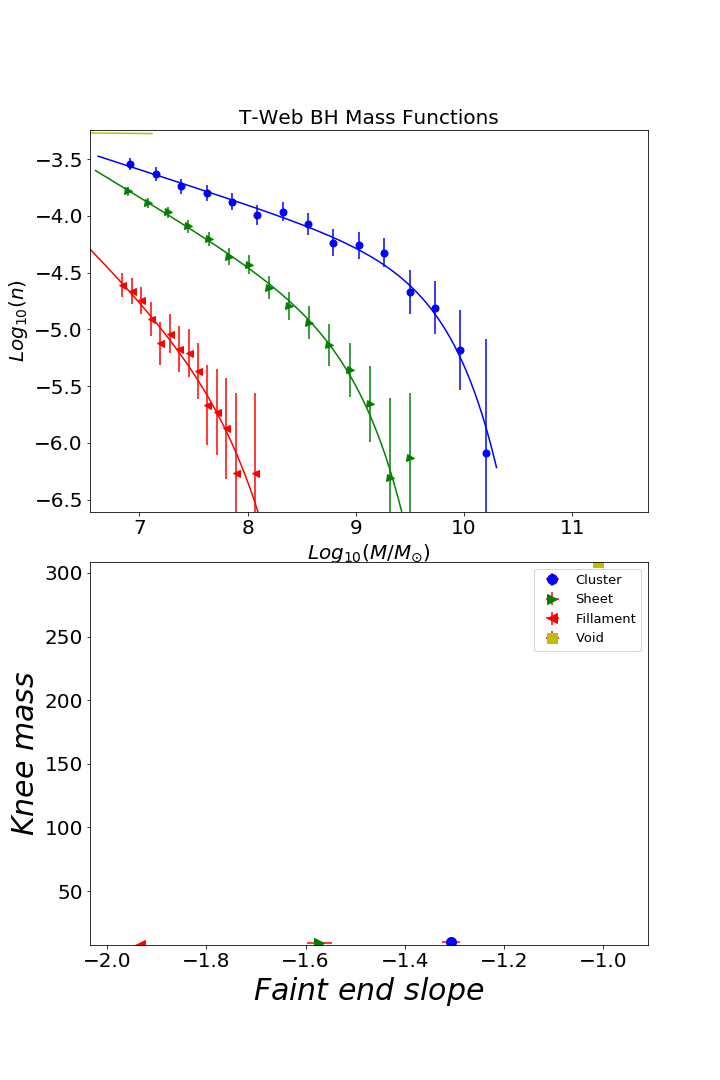
\includegraphics[width=\columnwidth]{./pics/T-Web_BH.png}
    \caption{\textbf{Upper side}: Schechter fits of each BH mass function for each morphological environment characterized by the T-Web algorithm proposed by Forero et al.\textbf{Down side}: Knee-mass $m_\ast$ and the faint end slope $\alpha$ values obtained from the Schechter fits for each curve shown above.}
    \label{fig:TwebBH}
\end{figure}

% Example table
\begin{table}
	\centering
	\caption{This is an example table. Captions appear above each table.
	Remember to define the quantities, symbols and units used.}
	\label{tab:example_table}
	\begin{tabular}{lccr} % four columns, alignment for each
		\hline
		A & B & C & D\\
		\hline
		1 & 2 & 3 & 4\\
		2 & 4 & 6 & 8\\
		3 & 5 & 7 & 9\\
		\hline
	\end{tabular}
\end{table}


\section{Conclusions}

The last numbered section should briefly summarise what has been done, and describe
the final conclusions which the authors draw from their work.

\section*{Acknowledgements}

The Acknowledgements section is not numbered. Here you can thank helpful
colleagues, acknowledge funding agencies, telescopes and facilities used etc.
Try to keep it short.

%%%%%%%%%%%%%%%%%%%%%%%%%%%%%%%%%%%%%%%%%%%%%%%%%%

%%%%%%%%%%%%%%%%%%%% REFERENCES %%%%%%%%%%%%%%%%%%

% The best way to enter references is to use BibTeX:

%\bibliographystyle{mnras}
%\bibliography{example} % if your bibtex file is called example.bib


% Alternatively you could enter them by hand, like this:
% This method is tedious and prone to error if you have lots of references
\begin{thebibliography}{99}
\bibitem[\protect\citeauthoryear{Author}{2012}]{Author2012}
Author A.~N., 2013, Journal of Improbable Astronomy, 1, 1
\bibitem[\protect\citeauthoryear{Others}{2013}]{Others2013}
Others S., 2012, Journal of Interesting Stuff, 17, 198
\end{thebibliography}

%%%%%%%%%%%%%%%%%%%%%%%%%%%%%%%%%%%%%%%%%%%%%%%%%%

%%%%%%%%%%%%%%%%% APPENDICES %%%%%%%%%%%%%%%%%%%%%

\appendix

\section{Some extra material}

If you want to present additional material which would interrupt the flow of the main paper,
it can be placed in an Appendix which appears after the list of references.

%%%%%%%%%%%%%%%%%%%%%%%%%%%%%%%%%%%%%%%%%%%%%%%%%%


% Don't change these lines
\bsp	% typesetting comment
\label{lastpage}
\end{document}

% End of mnras_template.tex